\documentclass{article}

\usepackage[ngerman]{babel}
\usepackage[utf8x]{inputenc}
\usepackage[T1]{fontenc}
\usepackage{lmodern}
\usepackage{graphicx} 
\usepackage{subfigure}
\usepackage{geometry}
\geometry{a4paper, left=2.5cm, right=2.5cm, top=2.5cm, bottom=3cm}

\title{Bachelorarbeit\\
	Capture of an Indruder by Mobile Agents}
\author{Jens Harder}
\date{\today}


\begin{document}
	\maketitle
	\newpage
	
	\pagenumbering{arabic}.
	\tableofcontents
	
	\newpage
	
	\section{Einleitung}
Diese Bachelorarbeit ist aus einer Projektarbeit entstanden, welche im Semester 2014/15 stattgefunden hat.\\

In dieser Projektarbeit habe ich einen Algorithmus aus dem Paper "'Capture of an Intruder by Mobile Agents"' (BARRIÈRE L. et al. 2002) in einem Java-Applet visuell dargestellt und implementiert. Es handelt sich bei dem Algorithmus um eine Variante des sogenannten "'graph-searching problems"'.\\

Man kann sich das Problem anschaulich wie folgt vorstellen: Ein Einbrecher ist in das Netzwerk eingedrungen und soll nun von mobilen Agenten gesucht werden. Sowohl die Agenten, als auch der Einbrecher können sich nur auf den Kanten des Graphen bewegen. Der Algorithmus soll die minimale Anzahl der Agenten berechnen, sowie den Knoten angeben, wo die Agenten die Suche im Baum anfangen sollen (die sogenannte Homebase), ohne zu wissen, wo sich der Einbrecher befindet. Je nachdem welcher Knoten als Homebase ausgewählt wird, kann sich die benötigte Anzahl an Agenten evt. ändern.\\

Da dieses Problem NP-Vollständig auf auf allgemeinen Graphen ist, werden sowohl im Paper, als auch in dieser Bachelorarbeit, nur Bäume betrachtet. Dadurch ist es möglich, einen linearen Algorithmus anzugeben, in dem die minimale Anzahl an Agenten sowie die dazugehörige Homebase berechnet werden.\\

Eine wichtige Eigenschaft, die wir aufrecht erhalten wollen ist die Monotonie. Diese bedeutet in diesem Fall, dass ein Knoten, den wir bereits dekontaminiert haben (kontrolliert, dass der Einbrecher dort nicht ist), nicht mehr kontaminiert werden kann (der Einbrecher bekommt keine Möglichkeit mehr in diesen Knoten zu gelangen). Um diese Eigenschaft zu gewährleisten müssen wir sogenannte Wachen aufstellen, die dekontaminierte Teilbäume vor dem Einbrecher schützen. Die einzelnen Teilbäume werden von den Agenten sukzessive kontrolliert, bis wir den ganzen Baum dekontaminiert haben.\\
\\
\\

Das Ziel dieser Bachelorarbeit ist es, auf Grundlage des in "'Capture of an Intruder by Mobile Agents"' (BARRIÈRE L. et al. 2002) beschriebenen Algorithmus weitere Problemstellungen zu betrachten. Ich untersuche im folgenden, wie sich ein Potenzial auf den Algorithmus auswirkt. Das Potenzial gibt an, um wieviel eine oder mehrere Kanten(-gewichte) reduziert werden können. Der Algorithmus soll in der Lage sein, dieses Potenzial zu nutzen, um die minimale Anzahl an Agenten, die gebraucht werden, um den ganzen Baum zu dekontaminieren, zu denken. Je nachdem, welche Kanten durch das Potenzial reduziert werden, ändert sich die minimale Anzahl der Agenten unterschiedliche stark. Es sollen nun eine optimale Verteilung an Kanten angegeben werden, um die Agentenzahl möglichst stark zu reduzieren.\\



	
	\section{allg Problemstellung}
	
	\subsection{orginaler Algo}
	//aus dem paper
	
	\subsection{neue interpreatation}
	//wieso?
	
	\section{Das Potenzial-Problem}

\subsection{Spezialfall k = 1}
//algo angeben, wieso ist er liniear? wieso korrekt?\\


Die Idee des Algorithmus ist es, zu protokollieren, welche Kante(n) für welche Knoten von Bedeutung ist:\\

Jeder Knoten berechnet im Algorithmus von BARRIÈRE L. et al. die minimale Anzahl von Agenten und jede Knoten hat mindestens eine Kante von der seine Agentenanzahl von abhängt.

\subsection{Potenzial auf einer Kante mit k > 1}

Um das Problem des Potenzials etwas zu erweitern, betrachte ich im folgenden Abschnitt Potenziale größer 1, allerdings mit der Einschränkung, dass man das gesamte Potenzial k nur auf einer Kante einsetzen darf.

Es fällt zunächst auf, dass man nicht garantieren kann, dass sich die Anzahl der benötigten Agenten auf allen Bäumen reduzieren lässt. Hierbei spielt es auch keine Rolle, wie groß das Potenzial k ist, da allein die Eigenschaft, dass man das Potenzial nur auf einer Kante einsetzen kann, genügt, um ein Gegenbeispiel zu finden:

Da das Potenzial k beliebig groß ist, kann man eine Kante auf Kantengewicht 1 setzen, man dadurch das größtmögliche Potenzial ausnutzt. Trotzdem ist es nicht möglich bei folgendem Baum die Anzahl der Agenten zu reduzieren:

\begin{figure}[h]
	\subfigure[alle Kanten haben Gewicht 4. Alle Knoten benötigen mindestens 8 Agenten.]{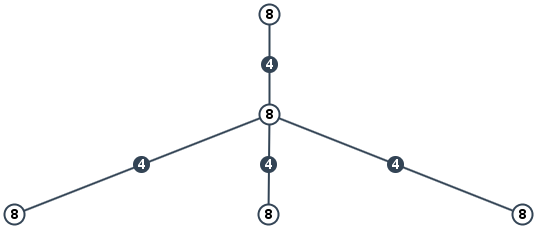
\includegraphics[width=0.49\textwidth]{bilder/abb1.png}} 
	\hfill
	\subfigure[eine Kante wurde auf Gewicht 1 geduziert, alle anderen haben weiterhin Gewicht 4. Alle Knoten benötigen trotzdem mindestens 8 Agenten.]{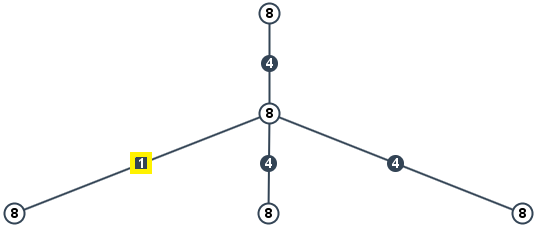
\includegraphics[width=0.49\textwidth]{bilder/abb2.png}} 
	\caption{Beispiel, dass Verringerung auf einer Kante nicht zu einer Verringerung der notwendigen Agenten führen muss} 
\end{figure} 

TODO:\\
//überlegung: woran sieht man, ob man die Agentenanzahl verringern kann?\\
//algorithmus angeben, welche kante ausgesucht wird?\\

\subsection{Potenzial verteilen mit k > 1}
	
	\section{cooperative gruppe}
	// wird das behandelt???
	
	\section{Fazit}
	
	
\end{document}
